\documentclass{standalone}
\usepackage{tikz}
\usetikzlibrary{calc, shapes, patterns}

\begin{document}
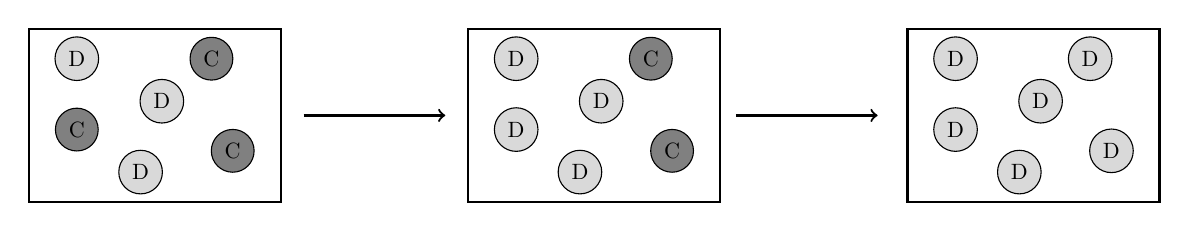
\begin{tikzpicture}[scale=.9]
    \node (Base) at (-.1, 0) [rectangle, draw=black, thick,
    minimum width=3.2cm, minimum height=2.2cm] {};
	\node (A1) at (-.3, -.8)  [circle, scale=0.80, draw=black, fill=gray!30] {D};
	\node (A2) at (-1.2, .8)  [circle, scale=0.80, draw=black, fill=gray!30] {D};
	\node (A3) at (0, .2)     [circle, scale=0.80, draw=black, fill=gray!30] {D};
	\node (B1) at (-1.2, -.2) [circle, scale=0.80, draw=black, fill=gray!] {C};
	\node (B2) at (1, -.5)    [circle, scale=0.80, draw=black, fill=gray!] {C};
	\node (B3) at (.7, .8)    [circle, scale=0.80, draw=black, fill=gray!] {C};

	\draw [->, thick] (2, 0) -- (4, 0) node [above, pos=0.5] {};

    \node (Base) at ($(Base) + (6.2, 0)$) [rectangle, draw=black, thick,
    minimum width=3.2cm, minimum height=2.2cm] {};
	\node (A1) at ($(A1) + (6.2, 0)$) [circle, scale=0.80, draw=black, fill=gray!30] {D};
	\node (A2) at ($(A2) + (6.2, 0)$) [circle, scale=0.80, draw=black, fill=gray!30] {D};
	\node (A3) at ($(A3) + (6.2, 0)$) [circle, scale=0.80, draw=black, fill=gray!30] {D};
	\node (B1) at ($(B1) + (6.2, 0)$) [circle, scale=0.80, draw=black, fill=gray!30] {D};
	\node (B2) at ($(B2) + (6.2, 0)$) [circle, scale=0.80, draw=black, fill=gray!] {C};
	\node (B3) at ($(B3) + (6.2, 0)$) [circle, scale=0.80, draw=black, fill=gray!] {C};

	\draw [->, thick] (8.1, 0) -- (10.1, 0) node [above, pos=0.5] {};

    \node (Base) at ($(Base) + (6.2, 0)$) [rectangle, draw=black, thick,
    minimum width=3.2cm, minimum height=2.2cm] {};
	\node (A1) at ($(A1) + (6.2, 0)$) [circle, scale=0.80, draw=black, fill=gray!30] {D};
	\node (A2) at ($(A2) + (6.2, 0)$) [circle, scale=0.80, draw=black, fill=gray!30] {D};
	\node (A3) at ($(A3) + (6.2, 0)$) [circle, scale=0.80, draw=black, fill=gray!30] {D};
	\node (B1) at ($(B1) + (6.2, 0)$) [circle, scale=0.80, draw=black, fill=gray!30] {D};
	\node (B2) at ($(B2) + (6.2, 0)$) [circle, scale=0.80, draw=black, fill=gray!30] {D};
	\node (B3) at ($(B3) + (6.2, 0)$) [circle, scale=0.80, draw=black, fill=gray!30] {D};
\end{tikzpicture}
\end{document}
